\documentclass{WMAfg}

\usepackage[german]{babel}
\usepackage[T1]{fontenc}
\usepackage[latin9]{inputenc}
\usepackage{array}

\usepackage{amsmath}
\usepackage{graphicx}
\usepackage{units}

\renewcommand{\Fach}{Lehrgang CAS mittels Jupyter Notebooks}
\renewcommand{\Textart}{Lernsituation Blowerdoortest}

\def\un#1 (#2){\ensuremath{\unit[#1]{#2}}}
\def\unf#1 (#2/#3){\ensuremath{\unitfrac[#1]{#2}{#3}}}
\def\gc{\ensuremath{^{\circ}\,C}}
\def\ts#1_#2{\ensuremath{{#1}_{\text{#2}}}}

\begin{document}

\fbox{
  \parbox[][3cm][t]{7.5cm}{
    \raggedright
    \textbf{Aufgabe 1} \\
    Achten Sie darauf, das Kommentarzeichen vor dem Aufruf von
    
    \texttt{lx = np.linspace()}

    zu entfernen
  }
}
\hspace{\fill}
\fbox{
  \parbox[][3cm][t]{7.5cm}{
    \raggedright
    \textbf{Aufgabe 2}\\
    Vervollst�ndigen Sie die Skizze:
    
    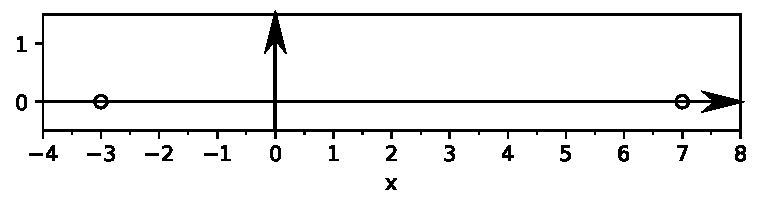
\includegraphics[width=\linewidth]{Hilfekarte_A2}
  }
}

\fbox{
  \parbox[][3cm][t]{7.5cm}{
    \raggedright
    \textbf{Aufgabe 3}\\
    Definieren Sie \texttt{lx} und den DataFrame in einer Zelle.

    Denken Sie an den Kontrollausdruck
  }
}
\hspace{\fill}
\fbox{
  \parbox[][3cm][t]{7.5cm}{
    \raggedright
    \textbf{Aufgabe 3}\\
    Vergleichen Sie den Plot-Befehl mit Aufgabe 1
  }
}

\fbox{
  \parbox[][3cm][t]{7.5cm}{
    \raggedright
    \textbf{Aufgabe 4}\\
    Beginnen Sie mit dem

    \texttt{lx = linspace())}

    Befehl. Setzen Sie \texttt{endpoint=False}.
  }
}
\hspace{\fill}
\fbox{
  \parbox[][3cm][t]{7.5cm}{
    \raggedright
    \textbf{Aufgabe 4}\\
    Wie lang ist ein Teilintervall?
  }
}

\fbox{
  \parbox[][3cm][t]{7.5cm}{
    \raggedright
    \textbf{Aufgabe 4}\\
    Was geschieht mit dem letzten Teilintervall?
  }
}
\hspace{\fill}
\fbox{
  \parbox[][3cm][t]{7.5cm}{
    \raggedright
    \textbf{Aufgabe 5}\\
    Nutzen Sie \texttt{retstep=True} im Aufruf von

    \texttt{np.linspace()}
  }
}

\fbox{
  \parbox[][3cm][t]{7.5cm}{
    \raggedright
    \textbf{Aufgabe 5}\\
    �berlegen Sie, wie viele Teilintervalle zur�ckgegeben werden.
  }
}
\hspace{\fill}
\fbox{
  \parbox[][3cm][t]{7.5cm}{
    \raggedright
    \textbf{Aufgabe 6}\\
    Testen Sie den

    \texttt{np.linspace()}

    Befehl mit \texttt{num=6} und erkl�ren Sie das Ergebnis.
  }
}

\fbox{
  \parbox[][3cm][t]{7.5cm}{
    \raggedright
    \textbf{Aufgabe 7}\\
    Was wissen Sie �ber \texttt{num}?
  }
}
\hspace{\fill}
\fbox{
  \parbox[][3cm][t]{7.5cm}{
    \raggedright
    \textbf{Aufgabe 7}\\
    Ermitteln Sie die Intervalll�nge und die Anzahl der Teilintervalle.
  }
}

\fbox{
  \parbox[][3cm][t]{7.5cm}{
    \raggedright
    T
  }
}
\hspace{\fill}
\fbox{
  \parbox[][3cm][t]{7.5cm}{
    \raggedright
    T
  }
}
\fbox{
  \parbox[][3cm][t]{7.5cm}{
    \raggedright
    T
  }
}
\hspace{\fill}
\fbox{
  \parbox[][3cm][t]{7.5cm}{
    \raggedright
    T
  }
}

\fbox{
  \parbox[][3cm][t]{7.5cm}{
    \raggedright
    T
  }
}
\hspace{\fill}
\fbox{
  \parbox[][3cm][t]{7.5cm}{
    \raggedright
    T
  }
}

\end{document}


%%% Local Variables: 
%%% mode: latex
%%% TeX-master: t
%%% End: 
